\documentclass[uplatex,dvipdfmx]{ujreport}

\author{片又佑美}
\title{ペンローズタイル張り上のライツアウトゲーム}

\usepackage{tikz,pgf,float}
\usepackage{amsmath}
\usepackage{amsfonts}
\usepackage{amssymb}

\begin{document}
\maketitle
\tableofcontents
\chapter{序}
\chapter{ペンローズタイル張り}
\section{ペンローズタイルについて}
ペンローズタイルとは、二種類の菱形で平面を充填したもので、イギリスの物理学者のロジャー・ペンローズが考案した。ペンローズタイルは他の平面充填とは異なり非周期的であるが、五回対称性がある。
準周期性を持つ。
\section{ペンローズタイルの構成}
ペンローズタイル張りを構成するためには
次のような三角形の分割、拡大操作を繰り返す。
タイプAの三角形は二辺の長さが$1$でそれに
挟まれる角度が$\frac{\pi}{5}$の三角形である。
タイプAの三角形を$\varphi$倍に拡大し、$\varphi:1$に分割したものが図2.1である。

以下では黄金比$\varphi$を以下のように定める。
\[
 \varphi^2 = \varphi + 1
\]
つまり、$\varphi$は
\begin{equation}
 \varphi =\frac{1+\sqrt{5}}{2}
\end{equation}
を満たす。


\begin{figure}[H]
  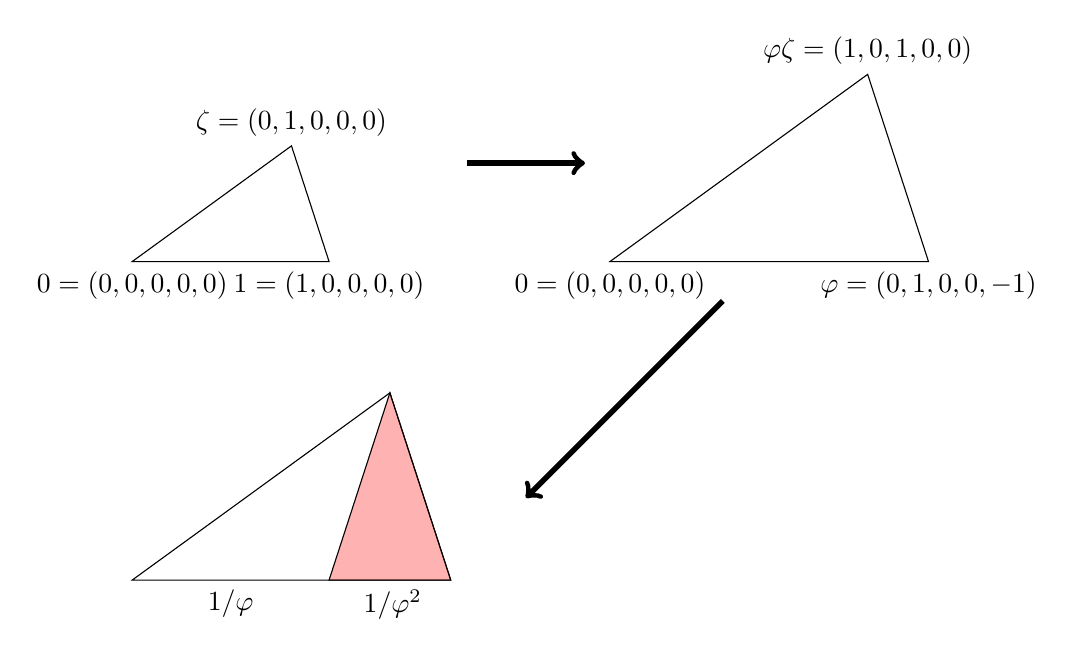
\begin{tikzpicture}[scale=2.5]
   \draw (0,0) -- (1,0) -- (36:1) -- cycle;
   \draw (0,0) node[below] {$0=(0,0,0,0,0)$};
   \draw (1,0) node[below] {$1=(1,0,0,0,0)$};
   \draw (36:1) node[above] {$\zeta=(0,1,0,0,0)$};
 
   \draw[->,line width=2] (1.7,0.5)--(2.3,0.5);
   
   \begin{scope}[scale=(sqrt(5)+1)/2,xshift=1.5cm]
    \draw (0,0) -- (1,0) -- (36:1) -- cycle; 
    \draw (0,0) node[below] {$0=(0,0,0,0,0)$};
    \draw (1,0) node[below] {$\varphi=(0,1,0,0,-1)$};
    \draw (36:1) node[above] {$\varphi\zeta=(1,0,1,0,0)$};
   \end{scope}
   \draw[->, line width=2] (3.0,-0.2)  -- (2.0,-1.2);
   \begin{scope}[scale=(sqrt(5)+1)/2,yshift=-1cm]
    \draw (0,0) -- (1,0) -- (36:1) -- cycle; 
    \draw[fill=red,fill opacity=0.3] ({(sqrt(5)-1)/2},0) -- (36:1) --(1,0) -- cycle;
    \draw ({(sqrt(5)-1)/4},0) node[below] {$1/\varphi$};
    \draw ({(sqrt(5)-1)/2+0.2},0) node[below] {$1/\varphi^2$};
   \end{scope}
 \end{tikzpicture} 
\caption{タイプAの三角形の分割}
\end{figure}

そして、タイプBの三角形は二辺の長さが$1$でそれに
挟まれる角度が$\frac{3}{5}\pi$の三角形である。
タイプBの三角形を$\varphi$倍に拡大し、$\varphi:1$に分割したものが図2.2である。

\begin{figure}[H]
  \begin{tikzpicture}[scale=2.5]
   \draw (0,0) -- (1,0) -- (36:{(sqrt(5)+1)/2}) -- cycle;
   \draw (0,0) node[below] {$0=(0,0,0,0,0)$};
   \draw (1,0) node[below] {$1=(1,0,0,0,0)$};
   \draw (36:{(sqrt(5)+1)/2}) node[above] {$\varphi\zeta=(1,0,1,0,0)$};
 
   \draw[->,line width=2] (1.7,0.5)--(2.3,0.5);
   
   \begin{scope}[scale=(sqrt(5)+1)/2,xshift=1.5cm]
    \draw (0,0) -- (1,0) -- (36:{(sqrt(5)+1)/2}) -- cycle; 
    \draw (0,0) node[below] {$0=(0,0,0,0,0)$};
    \draw (1,0) node[below] {$\varphi=(0,1,0,0,-1)$};
    \draw (36:{(sqrt(5)+1)/2}) node[above] {$\varphi^2\zeta=(0,2,0,1,-1)$};
   \end{scope}
   \draw[->, line width=2] (3.5,-0.3)  -- (2.5,-1.3);
   \begin{scope}[scale=(sqrt(5)+1)/2,yshift=-1.2cm]
    \draw (0,0) -- (1,0) -- (36:{(sqrt(5)+1)/2}) -- cycle; 
    \draw ({(sqrt(5)-1)/2},0) -- (36:1) --(1,0) -- cycle;
    \draw ({(sqrt(5)-1)/4},0) node[below] {$1/\varphi$};
    \draw ({(sqrt(5)-1)/2+0.2},0) node[below] {$1/\varphi^2$};
   \end{scope}
 \end{tikzpicture} 
\caption{タイプBの三角形の分割}
\end{figure}

平面$\mathbb{R}^2$を複素平面$\mathbb{C}$とみなすことで拡大や細分、回転といった操作を複素数同士の掛け算や足し算によって表現できる。
\[
  \zeta =\cos \frac{\pi}{5}+i \sin \frac{\pi}{5}
\]
と定める。この時、関係式
\[
  \zeta^5 =-1,   \zeta^{-1}=-\zeta^4
\]
$\varphi$と$\zeta$の関係式
\[
  \varphi =\zeta+\zeta^{-1}
\]
が成り立つ。従って
\begin{equation}
  \frac{1}{\varphi} =\varphi-1=\zeta+\zeta^{-1}-1
\end{equation}

が成り立つ。

ペンローズタイル張りに現れるタイルの頂点の座標は整数$5$個からなるベクトル$x=(x_0,x_1,x_2,x_3,x_4)$を用いて
\begin{equation}
 x_0+x_1\zeta+x_2\zeta^2+x_3\zeta^3+x_4\zeta^4
\end{equation}
と表現できる。

\begin{figure}[H]
 \begin{center}
 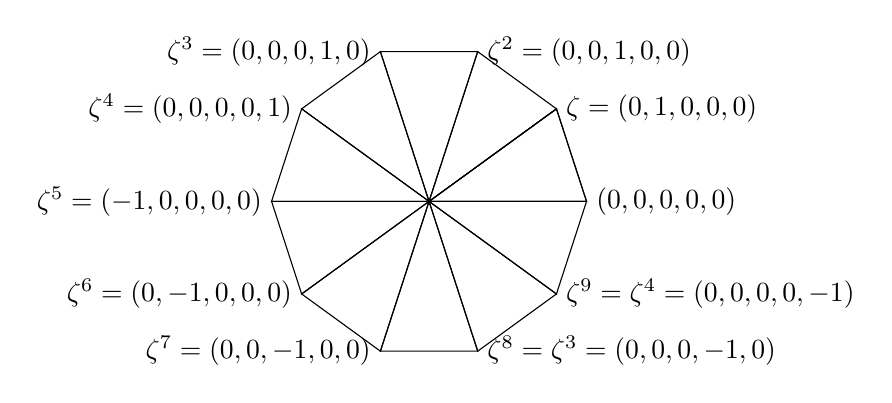
\begin{tikzpicture}[scale=2]
  \draw (0,0) -- (1,0) -- (36:1) -- cycle; 
  \draw (1,0) node[right] {$(0,0,0,0,0)$};
  \draw (36:1) node[right] {$\zeta=(0,1,0,0,0)$};
  \draw (72:1) node[right] {$\zeta^2=(0,0,1,0,0)$};
  \draw (108:1) node[left] {$\zeta^3=(0,0,0,1,0)$};
  \draw (144:1) node[left] {$\zeta^4=(0,0,0,0,1)$};
  \draw (180:1) node[left] {$\zeta^5=(-1,0,0,0,0)$};
  \draw (216:1) node[left] {$\zeta^6=(0,-1,0,0,0)$};
  \draw (252:1) node[left] {$\zeta^7=(0,0,-1,0,0)$};
  \draw (288:1) node[right] {$\zeta^8=\zeta^3=(0,0,0,-1,0)$};
  \draw (324:1) node[right] {$\zeta^9=\zeta^4=(0,0,0,0,-1)$};
  \draw (0,0) -- (1,0) -- (36:1) -- cycle;  
  \begin{scope}[rotate=36]
   \draw (0,0) -- (1,0) -- (36:1) -- cycle;  
  \end{scope}
  \begin{scope}[rotate=72]
   \draw (0,0) -- (1,0) -- (36:1) -- cycle;  
  \end{scope}
  \begin{scope}[rotate=108]
   \draw (0,0) -- (1,0) -- (36:1) -- cycle;  
  \end{scope}
  \begin{scope}[rotate=144]
   \draw (0,0) -- (1,0) -- (36:1) -- cycle;  
  \end{scope}
  \begin{scope}[rotate=180]
   \draw (0,0) -- (1,0) -- (36:1) -- cycle;  
  \end{scope}
  \begin{scope}[rotate=216]
   \draw (0,0) -- (1,0) -- (36:1) -- cycle;  
  \end{scope}
  \begin{scope}[rotate=252]
   \draw (0,0) -- (1,0) -- (36:1) -- cycle;  
  \end{scope}
  \begin{scope}[rotate=288]
   \draw (0,0) -- (1,0) -- (36:1) -- cycle;  
  \end{scope}
  \begin{scope}[rotate=324]
   \draw (0,0) -- (1,0) -- (36:1) -- cycle;  
  \end{scope}
 \end{tikzpicture}
  \caption{各タイルの頂点座標} 
 \end{center}
\end{figure}
\begin{itemize}
 \item [拡大]
       複素平面上の全体を$\varphi$倍する操作である。$\varphi=\zeta+\zeta^{-1}$
       なので、$x=(x_0,x_1,x_2,x_3,x_4)$とすると、
       \begin{equation}
	\begin{split}
	 \varphi x = 
	 &=(\zeta+\zeta^{-1})x \\
	 &=(\zeta+\zeta^{-1})(x_0,x_1,x_2,x_3,x_4)\\
	 &=(x_1-x_4) + (x_0+x_2)\zeta + (x_1+x_3)\zeta^2 + (x_2+x_4)\zeta^3 + (x_3-x_0)\zeta^4\\
	 &\mapsto(x_1-x_4, x_0+x_2, x_1+x_3, x_2+x_4, x_3-x_0)
	\end{split}
       \end{equation}
       と表せる。
       
 \item [細分]
       複素数xとyが与えられた時、それに対応する$5$次元座標を$x=(x_0,x_1,....,x_4)$,
       $y=(y_0,y_1,...,y_4)$とすると、線分$x-y$を$\varphi:1$に内分する点は
       \begin{equation}
	\frac{x+\varphi y}{\varphi+1}
       \end{equation}
       と表せる。
 \item [拡大後の細分]
       xとyを$\varphi$倍した点$\varphi x$と$\varphi y$を$\varphi:1$に内分する。
       \[
       \frac{(\varphi x)+\varphi(\varphi y)}{\varphi+1}
       \]
       である。$\varphi^2=\varphi+1$を用いると
       \[
       \frac{(\varphi x)+\varphi(\varphi y)}{\varphi^2}=\frac{1}{\varphi}x+y
       \]
       と変形できる。式(2.2)より
       \[
       \frac{1}{\varphi} x+y=(\varphi-1)x+y
       =\varphi x-x+y
       \]

\end{itemize}
式(2.4)を代入すると
\[
 (x_1-x_4, x_0+x_2, x_1+x_3, x_2+x_4, x_3-x_0)-x+y
 \]
と表せる。

タイプAのタイルに拡大細分を2度施すと以下のようになる。
\begin{figure}[H]
  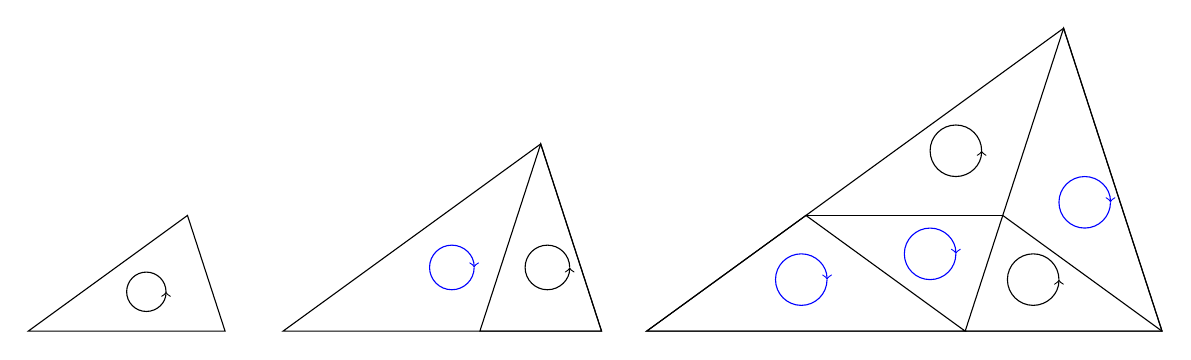
\begin{tikzpicture}[scale=2.5]
   \draw (0,0) -- (1,0) -- (36:1) -- cycle;
   \draw [->] (0.7,0.2) arc(0:360:0.1);
   \begin{scope}[scale=(sqrt(5)+1)/2,xshift=0.8cm]
    \draw (0,0) -- (1,0) -- (36:1) -- cycle; 
    \draw ({(sqrt(5)-1)/2},0) -- (36:1) --(1,0) -- cycle;
    \draw [->,blue] (0.6,0.2) arc(360:0:0.07);
    \draw [->] (0.9,0.2) arc(0:360:0.07);
   \end{scope}
   \begin{scope}[scale=(sqrt(5)+1)/2+1,xshift=1.2cm]
    \draw (0,0) -- (1,0) -- (36:1) -- cycle; 
    \draw ({(sqrt(5)-1)/2},0) -- (36:1) --(1,0) -- cycle;  
    \draw (0,0) -- ({(sqrt(5)-1)/2},0) -- (36:{2/(3+sqrt(5))}) -- cycle;
    \draw (1,0) -- +(144:{2/(3+sqrt(5))});
    \draw (36:{2/(3+sqrt(5))}) -- +(0:{2/(3+sqrt(5))});
    \draw [->,blue] (0.35,0.1) arc(360:0:0.05);
    \draw [->,blue] (0.6,0.15) arc(360:0:0.05);
    \draw [->] (0.65,0.35) arc(0:360:0.05);
    \draw [->,blue] (0.9,0.25) arc(360:0:0.05);
    \draw [->] (0.8,0.1) arc(0:360:0.05);
    
    
   \end{scope}  
 \end{tikzpicture} 
\caption{タイプAのタイルに2度拡大細分を施した状態} 
\end{figure}

そして、初期配置はタイプAのタイルを10枚円形になるように並べる。
ここでは、1枚おきに向きが反転するようにタイルを配置する。
つまり、タイプAのタイルを表向き、裏向きの交互に配置する。
\begin{figure}[H]
 \begin{center}
 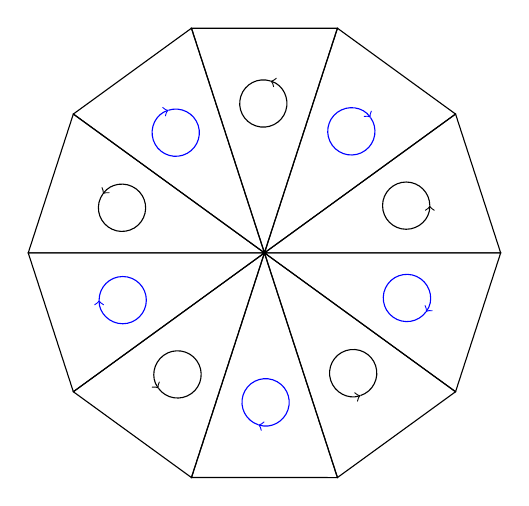
\begin{tikzpicture}[scale=3]
   \draw (0,0) -- (1,0) -- (36:1) -- cycle;
   \draw [->] (0.7,0.2) arc(0:360:0.1);
  \begin{scope}[rotate=36]
   \draw (0,0) -- (1,0) -- (36:1) -- cycle;
    \draw [->,blue] (0.7,0.2) arc(360:0:0.1);
  \end{scope}
  \begin{scope}[rotate=72]
   \draw (0,0) -- (1,0) -- (36:1) -- cycle;
   \draw [->] (0.7,0.2) arc(0:360:0.1);  
  \end{scope}
  \begin{scope}[rotate=108]
   \draw (0,0) -- (1,0) -- (36:1) -- cycle;
   \draw [->,blue] (0.7,0.2) arc(360:0:0.1);
  \end{scope}
  \begin{scope}[rotate=144]
   \draw (0,0) -- (1,0) -- (36:1) -- cycle;
    \draw [->] (0.7,0.2) arc(0:360:0.1);
  \end{scope}
  \begin{scope}[rotate=180]
   \draw (0,0) -- (1,0) -- (36:1) -- cycle;
   \draw [->,blue] (0.7,0.2) arc(360:0:0.1);
  \end{scope}
  \begin{scope}[rotate=216]
   \draw (0,0) -- (1,0) -- (36:1) -- cycle;
    \draw [->] (0.7,0.2) arc(0:360:0.1);
  \end{scope}
  \begin{scope}[rotate=252]
   \draw (0,0) -- (1,0) -- (36:1) -- cycle;
   \draw [->,blue] (0.7,0.2) arc(360:0:0.1);
   \end{scope}
  \begin{scope}[rotate=288]
   \draw (0,0) -- (1,0) -- (36:1) -- cycle;
    \draw [->] (0.7,0.2) arc(0:360:0.1);
  \end{scope}
  \begin{scope}[rotate=324]
   \draw (0,0) -- (1,0) -- (36:1) -- cycle;
   \draw [->,blue] (0.7,0.2) arc(360:0:0.1);
  \end{scope}
  \end{tikzpicture}
 \end{center}
 \caption{初期状態} 
\end{figure}

これに拡大細分を1回適用すると次のようになる。
\begin{figure}[H]
\begin{center}
  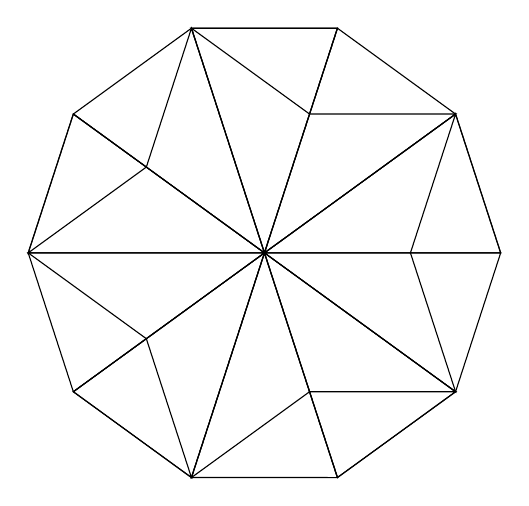
\begin{tikzpicture}[scale=3]
  \draw (0,0) -- (1,0) -- (36:1) -- cycle; 
  \draw ({(sqrt(5)-1)/2},0) -- (36:1) --(1,0) -- cycle;
  \begin{scope}[rotate=36]
   \draw (0,0) -- (1,0) -- (36:1) -- cycle; 
   \draw (0,0) -- (36:{(sqrt(5)-1)/2}) --(1,0) -- cycle;
  \end{scope}
  \begin{scope}[rotate=72]
   \draw (0,0) -- (1,0) -- (36:1) -- cycle;
    \draw ({(sqrt(5)-1)/2},0) -- (36:1) --(1,0) -- cycle;
  \end{scope}
  \begin{scope}[rotate=108]
   \draw (0,0) -- (1,0) -- (36:1) -- cycle;
   \draw (0,0) -- (36:{(sqrt(5)-1)/2}) --(1,0) -- cycle;
  \end{scope}
  \begin{scope}[rotate=144]
   \draw (0,0) -- (1,0) -- (36:1) -- cycle; 
    \draw ({(sqrt(5)-1)/2},0) -- (36:1) --(1,0) -- cycle;
  \end{scope}
  \begin{scope}[rotate=180]
   \draw (0,0) -- (1,0) -- (36:1) -- cycle;
   \draw (0,0) -- (36:{(sqrt(5)-1)/2}) --(1,0) -- cycle;
  \end{scope}
  \begin{scope}[rotate=216]
   \draw (0,0) -- (1,0) -- (36:1) -- cycle;
   \draw ({(sqrt(5)-1)/2},0) -- (36:1) --(1,0) -- cycle;
  \end{scope}
  \begin{scope}[rotate=252]
   \draw (0,0) -- (1,0) -- (36:1) -- cycle; 
   \draw (0,0) -- (36:{(sqrt(5)-1)/2}) --(1,0) -- cycle;
   \end{scope}
  \begin{scope}[rotate=288]
   \draw (0,0) -- (1,0) -- (36:1) -- cycle;
   \draw ({(sqrt(5)-1)/2},0) -- (36:1) --(1,0) -- cycle;
  \end{scope}
  \begin{scope}[rotate=324]
   \draw (0,0) -- (1,0) -- (36:1) -- cycle;
   \draw (0,0) -- (36:{(sqrt(5)-1)/2}) --(1,0) -- cycle;
  \end{scope}
  \end{tikzpicture}
 \end{center}
 \caption{初期状態に拡大細分を1度施した状態} 
\end{figure}

 
\chapter{ライツアウト}
\section{ライツアウトのルール}
ライツアウトは格子状に並んだライトを全て消灯させるゲームである。
それぞれライトはボタンになっており、あるボタンを押すとそのライト自身と
隣接するライトのオン・オフが反転する仕組みである。\\
いくつかのライトがオンの状態で始まり、何度かボタンを押し全てのライトをオフにすれば終了である。
ライツアウトは様々なバリエーションを作ることができ、もっと大きい格子状や多角形などでも同じルールでゲームを行うことができる。
 \begin{figure}[H]
  \begin{center}
  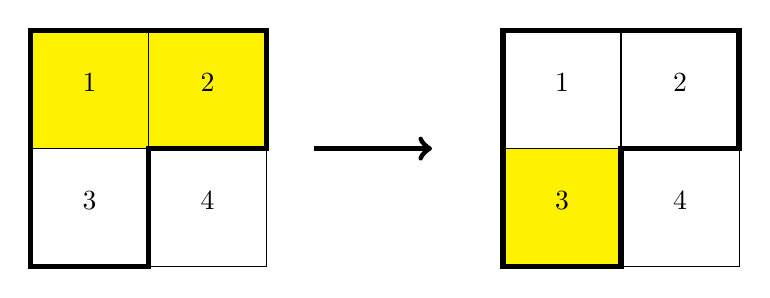
\begin{tikzpicture}[scale=3]
   \draw[fill=yellow] (0,0.5) -- (0,1) -- (0.5,1) -- (0.5,0.5) -- cycle;
   \draw[fill=yellow] (0.5,0.5) -- (0.5,1) -- (1,1) -- (1,0.5) -- cycle;
   \draw (0,0) -- (0.5,0) -- (0.5,0.5) -- (0,0.5) -- cycle;
   \draw (0.5,0) -- (1,0) -- (1,0.5) -- (0.5,0.5) -- cycle;

   \draw[line width=2] (0,0) --(0.5,0) --  (0.5,0.5) -- (1,0.5) -- (1,1) -- (0,1) -- cycle;
   \draw (0.25,0.7) node[above] {$1$};
   \draw (0.75,0.7) node[above] {$2$};
   \draw (0.25,0.2) node[above] {$3$};
   \draw (0.75,0.2) node[above] {$4$};
   \draw[->,line width=2] (1.2,0.5) -- (1.7,0.5);
   \begin{scope}[xshift=2cm]
   \draw (0,0.5) -- (0,1) -- (0.5,1) -- (0.5,0.5) -- cycle;
   \draw (0.5,0.5) -- (0.5,1) -- (1,1) -- (1,0.5) -- cycle;
   \draw[fill=yellow] (0,0) -- (0.5,0) -- (0.5,0.5) -- (0,0.5) -- cycle;
   \draw (0.5,0) -- (1,0) -- (1,0.5) -- (0.5,0.5) -- cycle;
    
    \draw[line width=2] (0,0) --(0.5,0) --  (0.5,0.5) -- (1,0.5) -- (1,1) -- (0,1) -- cycle;
    \draw (0.25,0.7) node[above] {$1$};
    \draw (0.75,0.7) node[above] {$2$};
    \draw (0.25,0.2) node[above] {$3$};
    \draw (0.75,0.2) node[above] {$4$};
  \end{scope}
  \end{tikzpicture}
  \caption{2$\times$2のライツアウト(1のライトを押した様子)} 
  \end{center}
 \end{figure}

\section{$p$元体\,$\mathbb{F}_p$について}
整数$a,b$と素数$p$に対し、$a-b$が$p$で割り切れるとき、
「$a$と$b$は$p$を法として合同である」といい、
\[
 a \equiv b\  (mod\ p)
\]
と表す。
そこで、$p$を法として合同な整数同士を一つのグループにまとめると、余り$0,\ 1,\ ...\ p-1$に分けることができる。
整数$\mathbb{Z}$が$p$個のグループに分けられ、この$p$個の集合が$p$元体$\mathbb{F}_p$である。
つまり、整数$\mathbb{Z}$を合同という同値関係で割って得られる商集合を$p$元体といい、
$\mathbb{F}_p$と書く。$\mathbb{Z}$は無限個の元があるのに対して、$\mathbb{F}_p$は
$p$個しか元を持たない。
\[
 \mathbb{F}_p=\{\{np|n \subseteq \mathbb{Z}\},\{1+np|n \subseteq \mathbb{Z}\}, ... ,\{(p-1)+np|n \subseteq \mathbb{Z}\}\}
\]
と書くことができ、
\[
 \mathbb{F}_p=\{[0],[1],...,[p-1]\}
\]
とも表現できる。

\section{デジタル表現}
ライツアウトのオン・オフの状態をデジタル表現に直す。
$2 \times 2$の格子状のライツアウトに対して
左上から図3.1のようにライトの場所に番号をつける。
オンの状態を$1$、オフの状態を$0$と表すことにすると
図の3.1で表した盤面をベクトルで$(1,\ 1,\ 0,\ 0)$と表現でき、
ライツアウトも$0$と$1$からなる$2$元体$\mathbb{F}_2$と考えられる。\\

そのため、それぞれの数字が$2$で割った余りだと考えると以下の式が成り立つ。
これより$1$回押すとオンの状態になり、$2$回以上押しても意味がないことがわかる。
また、どの順番で押すかはゲームには関係ないと言える。

 \begin{equation}
  \begin{split}
    0+1=1\\
   1+1=0  
  \end{split}
 \end{equation}

ここで$1$のボタンを押した場合を考える。
現在の盤面は
\[
 B=(1,1,0,0)
\]
であり、ボタン$1$を押すということは$B$に
\[
 A_1=(1,1,1,0)
\]
を足すことと同じである
$B$に状態$A_1$を加えると
\[
 B+A_1=(0,0,1,0)
\]
となり、図3.1の結果と同じになる。

つまり、$2\times2$の格子状のライツアウトでは
初期状態$B=(b_1,b_2,b_3,b_4)$に押した分だけボタン$A_i$を加えていくことになる。
状態$B$から$1$と$2$のボタンを押すということは、$B+A_1+A_2$ということだ。

そこで、$i$番目のボタンを押す場合は$x_i=1$、押さない場合は$x_i=0$とすると
\[
 x_1A_1+x_2A_2+x_3A_3+x_4A_4+B
\]
従って、ライツアウトは初期状態$B$に対して
\begin{equation}
  x_1A_1+x_2A_2+x_3A_3+x_4A_4+B=0
\end{equation}
を満たす$X=(x_1,x_2,x_3,x_4)$を求めるゲームである。

\section{ライツアウトの解法}
ライツアウトを解くと言うことは式3.2を解くことである。
\[
\begin{split}
  x_1A_1+x_2A_2+x_3A_3+x_4A_4+B=0\\
  x_1A_1+x_2A_2+x_3A_3+x_4A_4=-B
\end{split}
\]
$\mathbb{F}_2$であるので、式3.1より$1=-1$である。これを用いると
\begin{equation}
 x_1A_1+x_2A_2+x_3A_3+x_4A_4=B
\end{equation}

となる。
$2$元体$\mathbb{F}_2$における上記の方程式を解くには掃き出し法を使う。
$1$を押すとオン・オフが反転する$A_1$は
\[
 A_1=(1\ 1\ 1\ 0)
\]
同様にして
\[
 A_2=(1\ 1\ 0\ 1)
\]
\[
 A_2=(1\ 0\ 1\ 1)
\]
\[
 A_2=(0\ 1\ 1\ 1)
\]となる。

式3.3を解くので、連立方程式の拡大係数行列は以下のようになる。
\[
  \left(
    \begin{array}{ccccc}
      1 & 1 & 1 & 0 & b_1 \\
      1 & 1 & 0 & 1 & b_2 \\
      1 & 0 & 1 & 1 & b_3 \\
      0 & 1 & 1 & 1 & b_4
    \end{array}
  \right)
\]
この拡大係数行列を$2$元体$\mathbb{F}_2$に注意しながら
掃き出し法で解くと、
\[
  \left(
    \begin{array}{ccccc}
     1 & 0 & 0 & 0 & b_1+b_2+b_3 \\
     0 & 1 & 0 & 0 & b_1+b_2+b_4\\
     0 & 0 & 1 & 0 & b_1+b_3+b_4 \\
     0 & 0 & 0 & 1 & b_2+b_3+b_4
    \end{array}
  \right)
\]
となり、求める解は
\[
 (x_1\ x_2\ x_3\ x_4) = (b_1+b_2+b_3\ \ b_1+b_2+b_4\ \ b_1+b_3+b_4\ \ b_2+b_3+b_4)
\]
従って初期状態$B=(1,1,0,0)$より、$X=(0,0,1,1)$となり、$2$番目と$3$番目のボタンを押せばよい。

実際に押してみると、図3.2のように全てのライトが消灯できる。
\begin{figure}[H]
  \begin{center}
  \begin{tikzpicture}[scale=3]
   \draw[fill=yellow] (0,0.5) -- (0,1) -- (0.5,1) -- (0.5,0.5) -- cycle;
   \draw[fill=yellow] (0.5,0.5) -- (0.5,1) -- (1,1) -- (1,0.5) -- cycle;
   \draw (0,0) -- (0.5,0) -- (0.5,0.5) -- (0,0.5) -- cycle;
   \draw (0.5,0) -- (1,0) -- (1,0.5) -- (0.5,0.5) -- cycle;

   \draw (0.25,0.7) node[above] {$1$};
   \draw (0.75,0.7) node[above] {$2$};
   \draw (0.25,0.2) node[above] {$3$};
   \draw (0.75,0.2) node[above] {$4$};
   \draw[->,line width=2] (1.1,0.5) -- (1.4,0.5);
   \draw (1.3,0.2) node[above] {$3$を押す};
   \begin{scope}[xshift=1.6cm]
   \draw (0,0.5) -- (0,1) -- (0.5,1) -- (0.5,0.5) -- cycle;
   \draw[fill=yellow] (0.5,0.5) -- (0.5,1) -- (1,1) -- (1,0.5) -- cycle;
   \draw[fill=yellow] (0,0) -- (0.5,0) -- (0.5,0.5) -- (0,0.5) -- cycle;
   \draw[fill=yellow] (0.5,0) -- (1,0) -- (1,0.5) -- (0.5,0.5) -- cycle;
    
    \draw[line width=2] (0,0) --(1,0) --  (1,0.5) -- (0.5,0.5) -- (0.5,1) -- (0,1) -- cycle;
    \draw (0.25,0.7) node[above] {$1$};
    \draw (0.75,0.7) node[above] {$2$};
    \draw (0.25,0.2) node[above] {$3$};
    \draw (0.75,0.2) node[above] {$4$};
    \draw[->,line width=2] (1.1,0.5) -- (1.4,0.5);
    \draw (1.3,0.2) node[above] {$4$を押す};
  \end{scope}
   \begin{scope}[xshift=3.2cm]
   \draw (0,0.5) -- (0,1) -- (0.5,1) -- (0.5,0.5) -- cycle;
   \draw (0.5,0.5) -- (0.5,1) -- (1,1) -- (1,0.5) -- cycle;
   \draw (0,0) -- (0.5,0) -- (0.5,0.5) -- (0,0.5) -- cycle;
   \draw (0.5,0) -- (1,0) -- (1,0.5) -- (0.5,0.5) -- cycle;

    \draw[line width=2] (0,0) --(1,0) --  (1,1) -- (0.5,1) -- (0.5,0.5) -- (0,0.5) -- cycle;
    \draw (0.25,0.7) node[above] {$1$};
    \draw (0.75,0.7) node[above] {$2$};
    \draw (0.25,0.2) node[above] {$3$};
    \draw (0.75,0.2) node[above] {$4$};
  \end{scope}
  \end{tikzpicture}
  \caption{2$\times$2のライツアウト(掃き出し法の解を確かめる)} 
  \end{center}
 \end{figure}
\section{解のないライツアウト}

\begin{thebibliography}{99}
  \bibitem{game} ゲームで大学数学入門―スプラウトからオイラー・ゲッターまで―\\
・安田彦健・2018
\end{thebibliography}

\end{document}

